\documentclass{acm_proc_10ptArticle-sp}
\usepackage[T1]{fontenc}
\usepackage{listings}

\begin{document}

\title{Final Assignment - Social Web}

\numberofauthors{3}
\author{
%
% The command \alignauthor (no curly braces needed) should
% precede each author name, affiliation/snail-mail address and
% e-mail address. Additionally, tag each line of
% affiliation/address with \affaddr, and tag the
%% e-mail address with \email.
\alignauthor Mihnea Dobrescu-Balaur\\
	\affaddr{2549278}\\
	\email{mihnea@linux.com}
\alignauthor Zilvinas Kucinskas\\
	\affaddr{2547940}\\
        \email{zil.kucinskas@gmail.com}
}

\date{28 March 2014}
\maketitle

\section{Introduction}

With the rise in popularity of the Web, everybody around the world produces content, from local bloggers to global news agencies. This means that the online medium is now full of content, and that is great. The Web embodies diversity and pluralism in opinions, making sure that anybody can find useful content. However, with this much content available, it can be difficult for people to keep track of the items that interest them the most. And because of the decentralised nature of the Web, it can be difficult to find relevant articles.

In order to solve these problems, websites started providing RSS\footnote{http://en.wikipedia.org/wiki/RSS} feeds and more advanced users have started following them. There are even online aggregators, like the recently closed Google Reader\footnote{http://www.google.com/reader/about/}, in which an user could add multiple RSS feeds that he or she is interested in, and then the website will keep track of new articles and display them in managed lists.

The problem with RSS and aggregators like Google Reader is that they are not so user friendly, having a dense interface, similar to a full webmail inbox. Also, they display the articles in a plain way, with lots of text. This all adds up to an overload of information to the user. More recent applications, like Feedly\footnote{http://feedly.com/} and Flipboard\footnote{https://flipboard.com/}, have taken a fresh approach of the problem. They create rich, magazine-like layouts for the articles, and they also help with content discovery, having predefined and curated “feeds” that the users can subscribe to.

We believe that we can take this idea a step further, and create a rich visual timeline, in which the media content (images and videos) take precedence over the text, removing everything but the headline. This timeline helps the users quickly get up to speed with the latest events and news from around the world, and when they find an article that is interesting, they can read it from the original source, with the original layout, in just one click.

Since there is no such thing as one size fits all, our application allows users to select what regions they are interested in, as well as what domains. So, for example, one user might be interested in Politics around the US, while another user might be interested in Tech news from Asia. Personalising a timeline is easy, and a user can store multiple timelines on his or her account.

\section{Structured data}

Our application has to include articles from all over the world, on all possible topics, and to cover this demand we decided to use, first and foremost, the RSS feeds of the main news agencies in the world. Wikipedia provides a list\footnote{http://en.wikipedia.org/wiki/List\_of\_news\_agencies/} of them, grouped by country. Besides news agencies, we also include information from prominent newsletters like the New York Times\footnote{http://www.nytimes.com/} and online publications like The Verge\footnote{http://www.theverge.com}.

Besides XML data (via RSS), we also use the Twitter API in order to get JSON data of the tweets related to any given article.

To enrich the user’s visual experience, besides the media from the original article, we use the Bing search API to find relevant images and videos, that we then later embed in the rendered story.

All the mentioned data sources and others (detailed in the Analysis section) get mixed in a pipeline that builds a JSON object representing the visual summary of the story that we want to render for the user. Then, using Web technologies we fetch the corresponding JSON files in the frontend application and render them, building the timeline.

\section{Data analysis}

In order to give the user an approximation about the impact of the story they are skimming, we use Sentiment140\footnote{http://www.sentiment140.com/} to perform sentiment analysis on the tweets that we found for that story. Since location is important for our application and for our users, we group the sentiment results by region. Figuring out where do the tweet authors live exactly is not trivial, since the majority of tweets does not contain location information. To solve this problem, we rely on the information that users share on their profile page. However, since that data is not structured at all, we have to reason about its text value and decide what region it represents. We do this using the Google Geocoding API\footnote{https://developers.google.com/maps/documentation/geocoding/}. 

We were interested to extend our application to allow the user to search for a topic, and then provide the user with summarized information about the news that are referenced in tweets, and the users' perception of the news. First of all, the application would display the most popular news articles on Tweeter, as well as the ones with negative or positive connotations. This allows the user to have a balanced view on the topic. An example summary of the search results for the topic 'Malaysia' is in Table \ref{table:summaryresults}. 

Upon extraction of the urls from the tweets, we observed that there were subsets of urls covering different topics. We employed word clustering based on co-occurence of the words in tweets, and used code\footnote{https://github.com/danielpreotiuc/trendminer-clustering} from the trend-miner project\footnote{http://www.trendminer-project.eu/} for this. By using this approach, we can identify different subtopics related to the search topic - for example different events that have occured or will occur in Malaysia. A first cluster that came up when analyzing the tweets on the 'Malaysia' topic was Fig. \ref{screenshot:cluster1}, which relates to the search for data regarding the recent airplane accident. We used the techniques described in \footnote{http://www.trendminer-project.eu/images/d3.2.1.pdf} to assign the articles to the word clusters. A subset of these articles can be seen in \ref{table:linkscluster1}. Another cluster identified within the 'Malaysia' data is \ref{screenshot:cluster2}, which relates to the upcoming formula 1 event. A subset of the links related to this cluster are in \ref{table:linkscluster2}. We think this analysis would allow the user to browse through the subtopics related to a topic, judge the main theme from the world cloud, and browse through the identified articles. Overall, we want to provide the user with a global perspective on the searched topic. 

However, due to time and technical constraints, we were not able to implement the topic search features. First of all, only for the data on the 'Malaysia' topic, we gathered data from the Tweet Streaming API over 12 hours, to have sufficient tweets for our analysis. Moreover, the trendminer clustering application is computation intensive, and requires Java and Matlab to be run. Nonetheless, if such an analysis would be feasible, we think it would provide an added value to the user news search.

\section{Zilvinas Kucinskas individual part - sentiment analysis and visualization}

\subsection{Rationale}

Our application not only provides information about hot topics, but also analyzes Twitter posts with each topic. It uses Twitter API to get tweets to each topic. It analyses those tweets using Sentiment140\footnote{http://www.sentiment140.com/} analysis. Some other services use simple keyword based approach to analyse the tweets, but this one uses classifiers built from machine learning algorithms. It can provide both the aggregated sentiments or assesment of an individual tweet. Aggregated information is provided directly on the site using pie diagram, and it is possible to query the service to get data in JSON format. Our application splits tweets by country and provides visualisation using jVectorMap\footnote{http://jvectormap.com/}. This API provides capabilities to generate custom maps or use existing ones. We use world map to provide visualisation of sentiments.

The main rationale behind this feature is providing users with approximation of the impact article gives user's globally. There is three variants of different opinions - positive, negative and neutral. Everytime application is refreshed - new tweets are gathered for each separate article and sentiment analysis is provided. 

According to Wikipedia\footnote{http://en.wikipedia.org/wiki/Data\_visualization}, the main purpose of data visualization is to communicate information. Based on article "\textbf{Why is data visualization so hot?}" \footnote{http://blog.visual.ly/why-is-data-visualization-so-hot/}, humans are able to interpret information way better if they see it visually, because huge amount of data can be transmitted to the brains through the optic nerve. Usually it's hard to understand the data looking only to numbers, but using data visualisation it is possible to see patterns and trends in the data way easier and faster \cite{kaidi}.

In my opinion, every text human reads could provide some impact on him, he may feel angry, scared, astonished, excited, neutral and so on. Usually, the more followers user has, the more it is influential to others. Sentiment analysis and visualisation feature provides our application users the opportunity to compare their sentiments to the ones in the Twitter social network. By splitting sentiments by country, we provide them the opportunity to find some patterns in the sentiment world map. Because each country has separate traditions and culture, people from different countriens feel differently about same topics. For example, occupation in Crimea is a really hot topic right now. By analysing sentiments, we were able to see that Russia has a positive sentiment regarding Crimea and for example France has more negative sentiment about it. So by having this information it is possible to make assumptions that Russia wants to occupy Crimea, and russian media is supporting it and that media from EU, France is against Crimea occupation. This can be shown in the Appendix figure \ref{screenshot:crimea}.

\subsection{Motivation}

Our application is oriented to people, who are interested in reading news articles, for users, who is keen to know what is happening around the world or in different domains of knowledge. By providing only pictures, videos and headline of an article, it is far more easier to search content to read. People can skim pages really fast and select which articles they want to read. They can also personalize their content by specifying which domain or regions he is interested in, also he has an opportunity to have several timelines. By clicking on specific article user gets redirected straight to the article in some online media source.

\subsection{Scoping}

Besides nice features our application also has some limitations. For example pictures and videos extracted from Bing could not always reflect the article, but we believe at least images and videos extracted directly from each online media source article is accurate. For example, there is a screenshot of an article in our application in this report Appendix figure \ref{screenshot:limitation}, which demonstrates this limitation. Also sentiment analysis could not be completely accurate. For example, tweets containing sarcasm can be evaluated completely opposite from it's initial sentiment. And almost always more than 50 percent tweets are evaluated as neutral. This is also a limitation, because variance between positive and negative sentiments is not so obvious.

\subsection{Evaluation}

Evaluation is really important thing in application growth and development. As applications need to be as much friendly and attractive for users, they need to change and adapt over time. First thing would be to look at the users, which are coming back and compare them to new users. Percentage of coming back user would be a good statistic of successfull application overall. This could be easily done by using Google Analytics\footnote{https://www.google.com/analytics}.

Also it would be nice to gather user's preferences and which articles he chooses to look at. It could be possible to analyze gathered data and make a list of most popular articles, and not so popular ones. By having this kind of information it would be possible to look at why people choose on article over another. It could be related with sentiments. It could be possible see if there are any patterns on sentiment analysis, which drives users to see one article over another.

\subsection{Future work}

How would you improve and further develop your application design if time  and efforts would permit?


\section{Mihnea Dobrescu-Balaur individual part}

\subsection{Individual study of a feature - content discovery}

In the following part of the report, we will discuss about \textbf{content discovery}, along with \textbf{clustering and correlation} by region, subject, tag etc.

This includes the way that the news articles are first fetched, then filtered and categorized, taking into account the preferences and specifics of every user.

The following sections will look at \textit{rationale} (the theory behind the feature and how it works), \textit{motivation} (why is this feature key to the application and how does it bring value to users), \textit{limitations} (and how they can be managed), \textit{evaluation} (metrics of quantifying the validation of the feature) and \textit{future work} (how could the application be improved).


\subsection{Rationale}

As presented in the introduction, the Web follows a decentralized model, having information floating everywhere around. Furthermore, the web started mostly \textit{schema-less}, meaning that even though the HTML markup has a structure and a syntax (that many authors don't respect 100\%), they don't provide any semantic value, making most of the content unstructured. More recent efforts, like schema.org\footnote{http://schema.org/} and microformats.org\footnote{http://microformats.org/} have tried to improve this situation, but there is still a long way to go.

Because of this, finding specific information around the Web is a nontrivial task. This is why many online news aggregators have employees that manually find and filter articles.

With our application, the intention is to completely automate this process. One way would be to use some very clever machine learning algorithms in order to come up with some classifiers that given a piece of content from the Web can decide what category it belongs to, in what geographic region the content is relevant, and (most importantly) if it is a quality article or not. Even though this approach is extremely interesting, it demands a large amount of resources (both in computing power and in human time), and it was not feasible for the scope of our project.

The other way to solve this problem is to use the work already done by other such algorithms or people. It is worth mentioning that this approach is only possible thanks to the development of the Social Web, together with Linked Data\footnote{http://linkeddata.org/}, that allow for machine-based discovery of content online.

The main data source for our applications are RSS feeds of news agencies (and other popular newspapers) around the world. RSS uses XML, and it makes use of semantic markup. Having an article in RSS format, it is easy to extract basic information like title, description and publish date. Some feeds, like the one from NY Times\footnote{http://www.nytimes.com} even provide categories in the markup, so we can know with no extra work that an article is, for example, about politics.

\begin{minipage}{\linewidth}
\begin{lstlisting}[language=XML, frame=single, caption=Example RSS feed, breaklines=true, captionpos=b]
<?xml version="1.0" encoding="UTF-8" ?>
<rss version="2.0">
<channel>
 <title>RSS Title</title>
 <description>This is an example of an RSS feed</description>
 <link>http://www.someexamplerssdomain.com/main.html</link>
 <lastBuildDate>Mon, 06 Sep 2010 00:01:00 +0000 </lastBuildDate>
 <pubDate>Mon, 06 Sep 2009 16:20:00 +0000 </pubDate>
 <ttl>1800</ttl>
 
 <item>
  <title>Example entry</title>
  <description>Here is some text containing an interesting description.</description>
  <link>http://www.wikipedia.org/</link>
  <guid>unique string per item</guid>
  <pubDate>Mon, 06 Sep 2009 16:20:00 +0000 </pubDate>
 </item>
 
</channel>
</rss>
\end{lstlisting}
\end{minipage}

We get the news agencies list from Wikipedia \footnote{http://en.wikipedia.org/wiki/List\_of\_news\_agencies}
, and the other newspapers and websites are added by our own judgment. Because the list of news agencies is clustered by region, it is trivial to decide in what regions the articles we find are relevant. This implies that we have to trust the news agencies for sharing relevant articles, and it is an assumption that we accept.

Thanks to the structured nature of the RSS feeds, we can find related articles, media and tweets using other APIs, like Bing search and Twitter search. We used Bing because it allows more queries for free than other competitors and that allowed us to experiment during development.

The data source for our application stays updated thanks to the pipeline of operations that put in place (discovering content, processing it, enhancing it with media and tweets, performing sentiment analysis and rendering) that monitors the mentioned RSS feeds of the upstream content channels.

It is worth mentioning that if we decide to add an extra type of data to the timeline, it is easy to plug it in into the existing architecture, thanks to the pipeline design.

\subsection{Motivation}

When choosing a theme for this assignment, we wanted to opt for an idea that would lead to a useful product, something that adds value to the modern day, always up to date, and always in a rush user. We thought about the benefits of the Social Web and of Linked Data, and we realized that one of the biggest benefits that are brought by this pair is enhanced knowledge. The World Wide Web is an enormous "place" that contains vast amounts of information, but finding the proper bits of information can be hard because of its big scale. The Social Web and Linked Data help in this problem because they empower search engine (and other automated tools) in partially understanding what items on the Web are about, what their semantics are.

Having this in mind, we decided to try to come up with a way that improves the way people get up to speed with the latest events around the world. Some read newspapers, some talk to their coworkers and find out what is happening, and only a few other use online tools like RSS readers or aggregators like Flipboard. We feel that we can raise the number of people who make use of the benefits of the Social Web by creating a web application that solves the same problem as skimming through a few newspapers.

The motivation for making this web application is that while not most people have really fast super smartphones or tablets or laptops, most people with access to technology also have Internet access, and so they can browse the Web. This meant that our application can reach a great number of people.

The other big decision was going for a visual timeline, in contrast to the current options that, as shown in the introduction, rely more on text. We feel that humans are visual entities, and following the saying that a picture is worth a thousand words, we think that we can make the experience of going through news faster by relying more on images than on full-page text.

We also decided not to affect the original content in any way, so when a user wants to read more about a story, we link them back to the original source. This is different than what other products do. For example, Flipboard creates a magazine layout out of the articles it aggregates. While the user experience is generally appealing, there are some times when the content doesn't properly fit the layout the application generates.

We hope that all these decisions together make up an accessible and easy to use web application that people around the world can use to get up to date to the events that interest them, regardless of the digital platform they are using to access the Internet.

\subsection{Limitations}

In order to save time and come up with a working application within the given time constraints, we made some choices that both helped us reach our goal faster and introduced some limitations.

The main limitation is the fact that we rely on other curated data sources, and that we don't do our own curation and discovery. This means that if a news agency that we trust releases some poor quality articles, we will also include them in the corresponding sections.

Another issue is the fact that we do not show content from social (micro) blogging websites like Medium\footnote{http://www.medium.com} and Tumblr\footnote{http://www.tumblr.com}. Many times, there are great popular articles on platforms like these, that people actively follow. Because we lack in this area, our application ends up more in the "news" end of the content spectrum.

It is worth mentioning that both limitations could be overcame, given enough time and resources. The first can be solved by using a custom classifier that could be built with an open source service such as Prediction.io\footnote{http://prediction.io/}. The second can be solved by just adding the RSS feeds of the mentioned services (both Medium and Tumblr provide RSS feeds), and writing some web scrapers for services that do not provide feeds.

Extended user testing would probably reveal other issues, as long as potential fixes to them. However, given the time in which we developed and tested the prototype, the before mentioned facts were the main limitations that we encountered.

\subsection{Evaluation}

Considering the fact that our application is Web based, we think that the regular website analytics are a good fit.

In this section, we will define the key metrics that are relevant for our evaluation, as well as explain why we chose them.

The number of \textbf{unique visitors} is defined as the total number of people (counted only once) that have visited the website. There are multiple aspects that take part of this calculation, but in essence different visitors are tracked by elements IP addresses, session data and cookies. Google provides\footnote{https://support.google.com/analytics/answer/2992042?hl=en} more information on this subject. This is relevant in order to figure out how many people are interested in the application. A high number of unique visitors means that there is genuine interest and that the idea is a valid one, satisfying a need. This does not necessarily measure if the execution (the application itself) is any good, just that the idea is valid.

The \textbf{average visit duration} is a measure in seconds of the total time a visitor spends on the website (regardless of the separate pages navigated). This is an approximated measure, but the technique was perfected over time, so it is reliable. This metric is relevant because it gives an idea about how the users interact with the website. A very low visit duration can be correlated with a high bounce rate (see below), and a very high visit duration can mean that information is hard to find. We don't know what the perfect balance is, but experimenting with the application and tracking the evolution of the average visit duration helps in improving the application's flow.

Another relevant metric is the \textbf{return rate}. It shows what percentage of visitors come back to the website, in a given time interval. So if ten people visit the site today, and then five of them will visit it again tomorrow, then the return rate for this period was 50\%. This metric complements the unique visitors count and is extremely useful, showing if the users like the web application. If they do, they return to the website. It is a simple metric with a high reward.

\textbf{Bounce rate} is defined as the percentage of visitors that just enter the website and leave. Because of the way current single page apps are set up, one could consider that the user of such an app never navigates to any page and such the site will have a high bounce rate. Current analyitcs tools have ways of avoiding this issue, in order to display relevant results. Wikipedia has more information\footnote{http://en.wikipedia.org/wiki/Bounce\_rate}. Studying bounce rate helps identifying visitors that are interested in the idea of the application (since they came to the page), but are not satisfied with the implementation and leave. Tracking the bounce rate helps in improving user retention.

\textbf{Visitor demographics} data provides information about what the age, interest and region of the website users. This insight helps us in tweaking our regional-based content, by identifying problems like "the sports content in the US is sub-average", or "the technology content in Japan is liked by our users, maybe we can find a similar source for a different region".

We believe that using the mentioned standard Website analytics metrics, we can track the evolution and user acquisition of the application. Common platforms like Google Analyitics\footnote{http://www.google.com/analytics/} offer the functionality we need at no cost. Also, implementing the tracking is easily done, by adding a small JavaScript snippet to the HTML code of the page.

A different kind of evaluation that would be relevant after the application reaches a larger amount of users is the performance evaluation. This includes analyses like response time measurement and memory usage.

The response time of a web application is important\footnote{http://www.nngroup.com/articles/response-times-3-important-limits/} in the user experience, since a website that takes too long to respond appears broken to users and they tend to leave.

Memory usage becomes relevant when scaling out the application, in order to require a smaller amount of servers.

However, we did not put strong accent on performance analysis in the beginning, since as long as there is not a large amount of users accessing the application, the response times are fast.

\subsection{Future work}

As mentioned in the Rationale section, the demonstrated application is a \textit{working prototype}, not close to the actual envisioned product. This was mainly because of the time and resources available at the moment. Even if we only developed a prototype, this has helped us realize what features are relevant and not, what limitations our idea has, and what we can do to improve it. There are a number of items that we would like to implement or improve, having the possibility.

First of all, right now we manually run the data aggregator program and then we upload the generated JSON file to the web server so that it can be rendered in the timeline. We would like to set up an automatic batch job that fetches the latest data, processes it and then exposes it to the frontend via an accessible API.

Adding more content types would also be helpful. For example, we think that adding videos alongside the images can enrich the users' experience. Another idea we have is to embed a few popular tweets about the given subjects into the timeline.

Having the possibility of geotagging the tweets that we display, it would be useful to further improve the sentiment analysis part of the application in order to allow the users to better visualize sentiment about articles around the world, and also see the statistics clustered by sources and categories.

At the moment, the Sentiment140\footnote{http://www.sentiment140.com/} API only supports English and Spanish, but our application targets people all around the world. We would like to improve the sentiment detection aspect in such a way that it would also support other languages. This could be done by using other services or by implementing a clever algorithm ourselves. An easy workaround would be to use the Twitter search API with the smileys support\footnote{https://dev.twitter.com/docs/using-search}, such that when looking for positive tweets we pass in ":)" and for negative tweets ":(".

Right now, the prototype shows world news. Since the data already supports it, we would like to allow the users to select what region they care about and have the frontend filter out articles only relevant to that region. If requested, we could also look into supporting multiple regions.

A similar approach can be done for categories, such that someone could set the timeline up so that they only see news about sports and technology.

We would like to implement a login system, probably using other providers (like OpenID\footnote{http://openid.net/}), in order to allow the users to have a profile within our application. This would enable the possibility of other features, like personalization.

Having a profile, users could personalize their timeline, for example by changing the theme, or the number and size of the thumbnails they want to see. Other settings like pagination, larger font size etc. can be added.

Furthermore, supporting region and category filtering (as described above), a user could save a configured timeline such that the next time he or she logs in to our application, the same timeline is already there, waiting to be browsed. In addition, there could be added support for multiple such configured timelines.

We know that we can't possibly include all the relevant news sources in the world, which is why another functionality that we think might be relevant is allowing the users to add their own data sources in the timelines. These can be saved per user profile, and if they lead to higher return rates, they could end up being shared between multiple users.

All in all, the above mentioned features would provide a complete experience that would allow new users to find everything they need in our application, as well as have the necessary features in order to make it possible for users of other news aggregators to migrate to our platform.




% The following two commands are all you need in the
% initial runs of your .tex file to
% produce the bibliography for the citations in your paper.
\bibliographystyle{abbrv}
\bibliography{final}

\newpage

%Appendix A
\onecolumn
\section{Appendix}

\ref{screenshot:reader}
\begin{figure}[H]
  \centering
  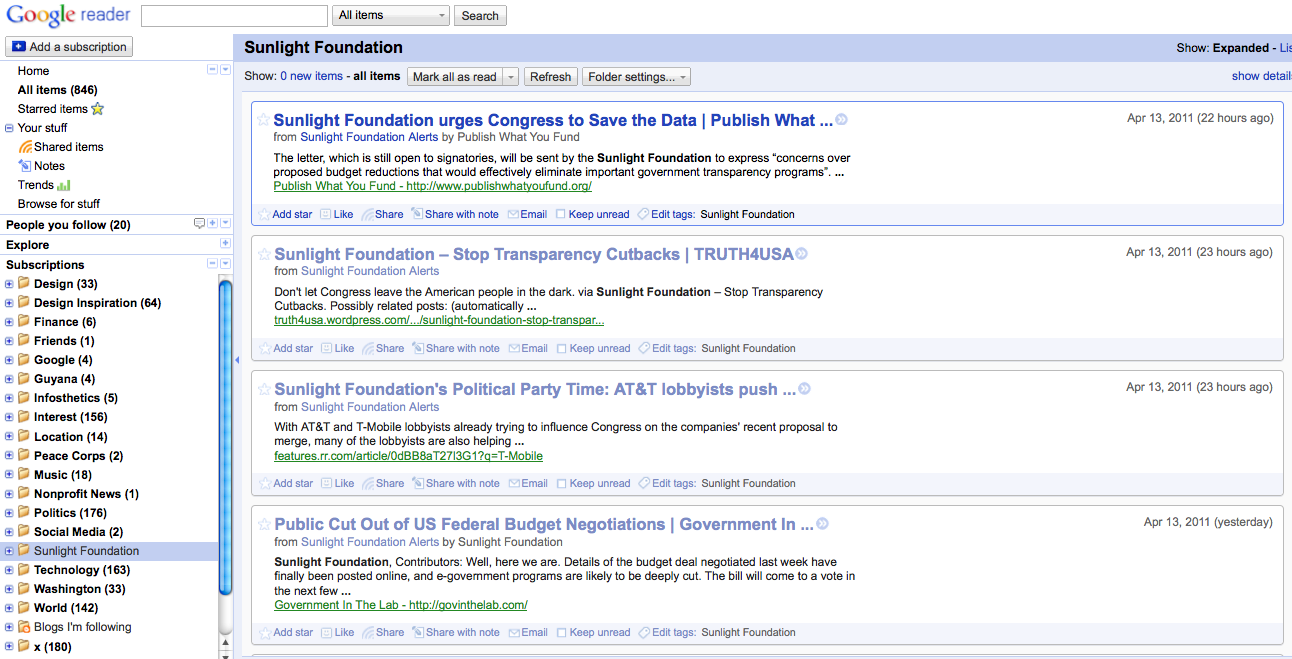
\includegraphics[width=0.9\linewidth]{img/Google-Reader.png}
  \caption{Google Reader screenshot}
  \label{screenshot:reader}
\end{figure}

\ref{screenshot:flipboard}
\begin{figure}[H]
  \centering
  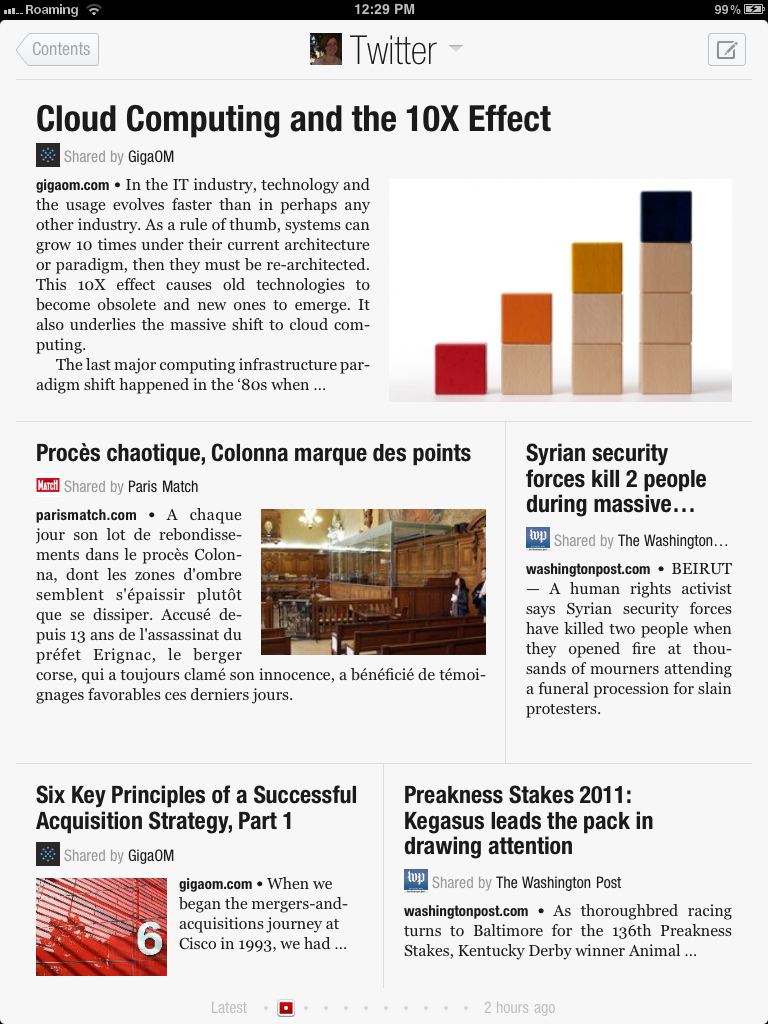
\includegraphics[width=0.9\linewidth]{img/flipboard-screenshot.png}
  \caption{Flipboard screenshot}
  \label{screenshot:flipboard}
\end{figure}

\ref{screenshot:timeline}
\begin{figure}[H]
  \centering
  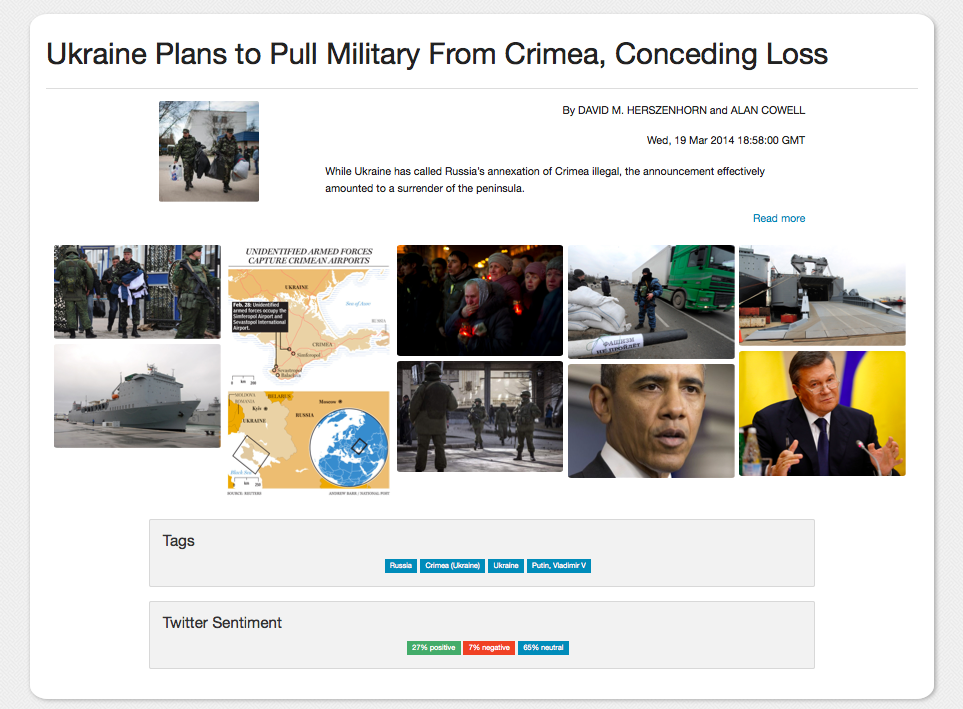
\includegraphics[width=0.9\linewidth]{img/timeline-item.png}
  \caption{Timeline item in our application}
  \label{screenshot:timeline}
\end{figure}

\ref{screenshot:coverage}
\begin{figure}[H]
  \centering
  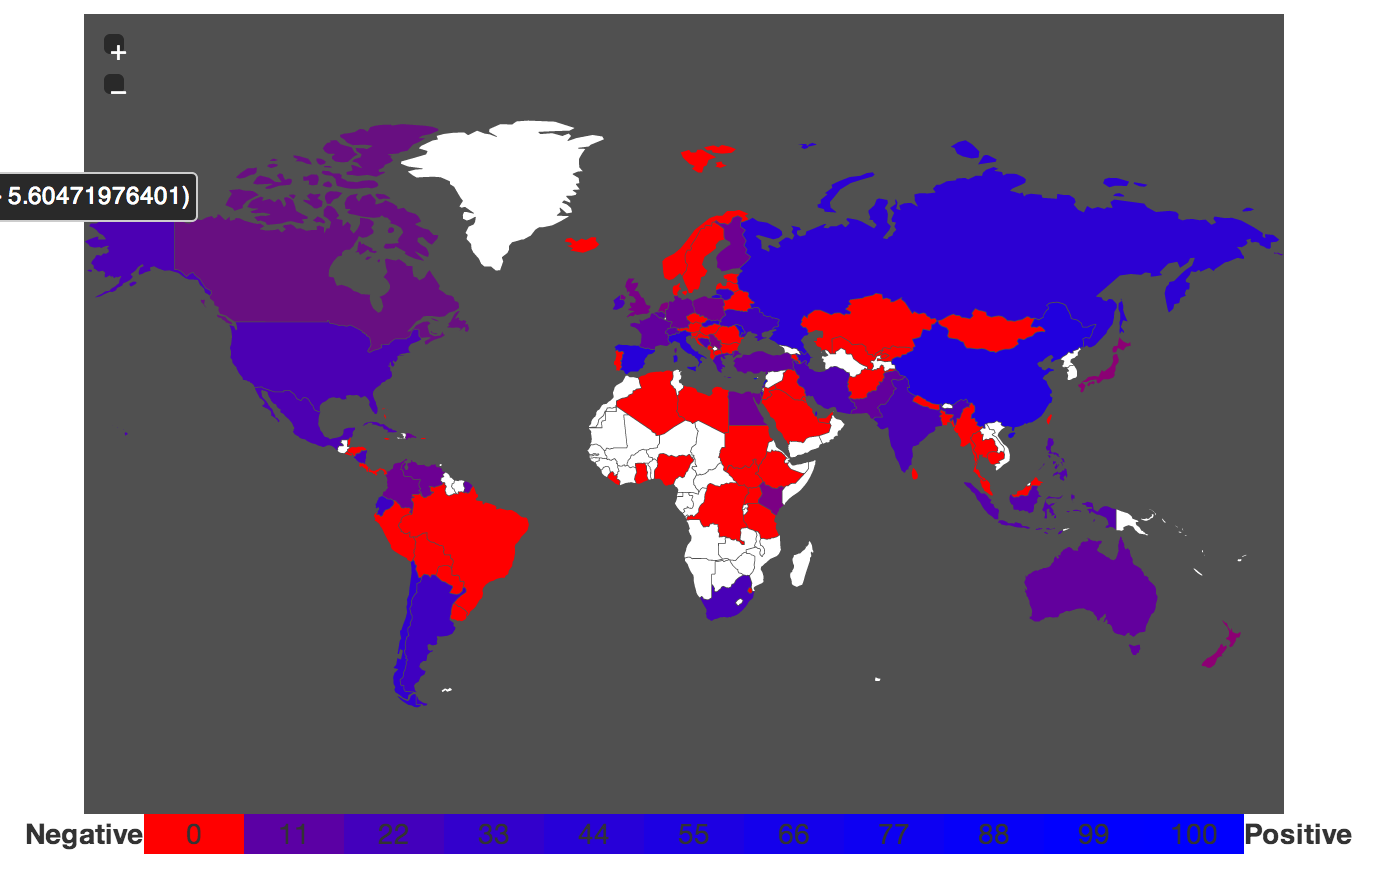
\includegraphics[width=0.9\linewidth]{img/media-coverage-polynomial.png}
  \caption{Media coverage visualization (polynomial)}
  \label{screenshot:coverage}
\end{figure}

\ref{screenshot:crimea}
\begin{figure}[H]
  \centering
  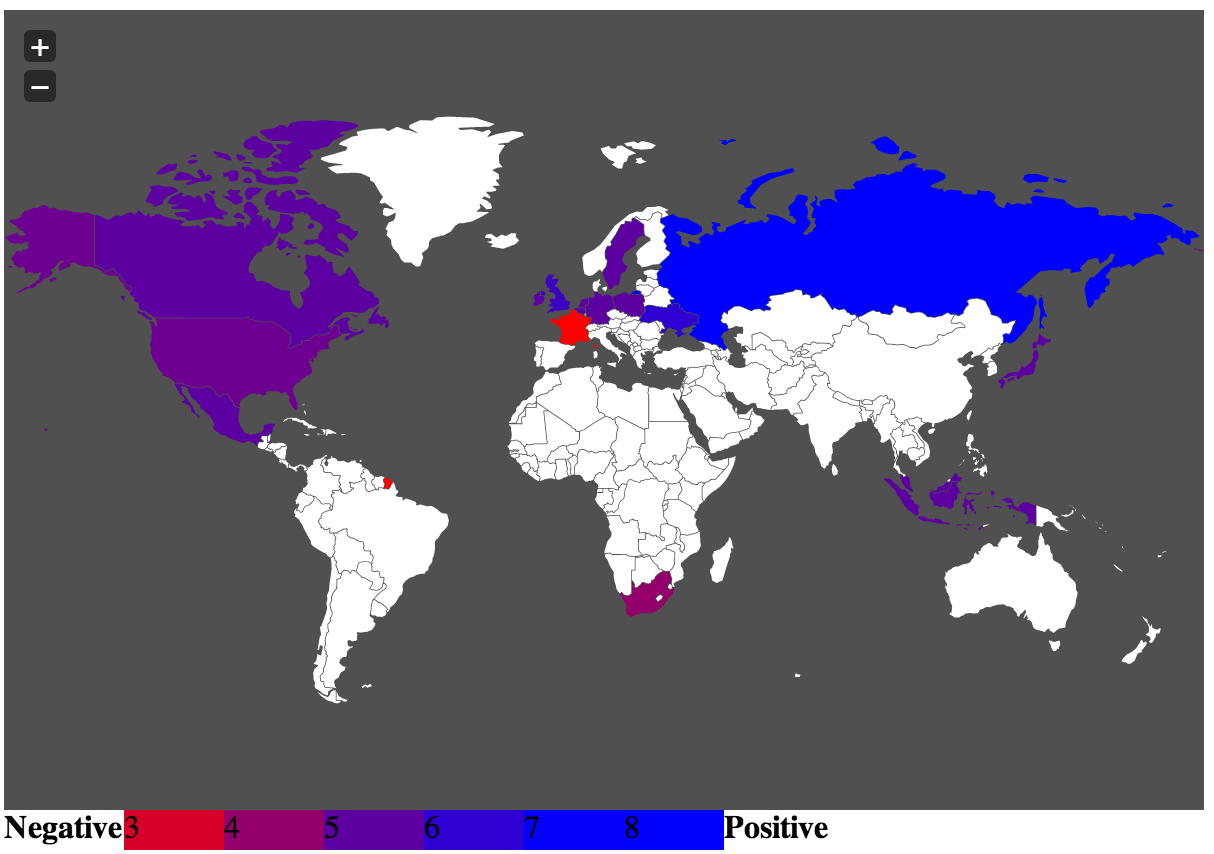
\includegraphics[width=0.9\linewidth]{img/crimea.png}
  \caption{Sentiment analysis about crimea topics}
  \label{screenshot:crimea}
\end{figure}

\ref{screenshot:limitation}
\begin{figure}[H]
  \centering
  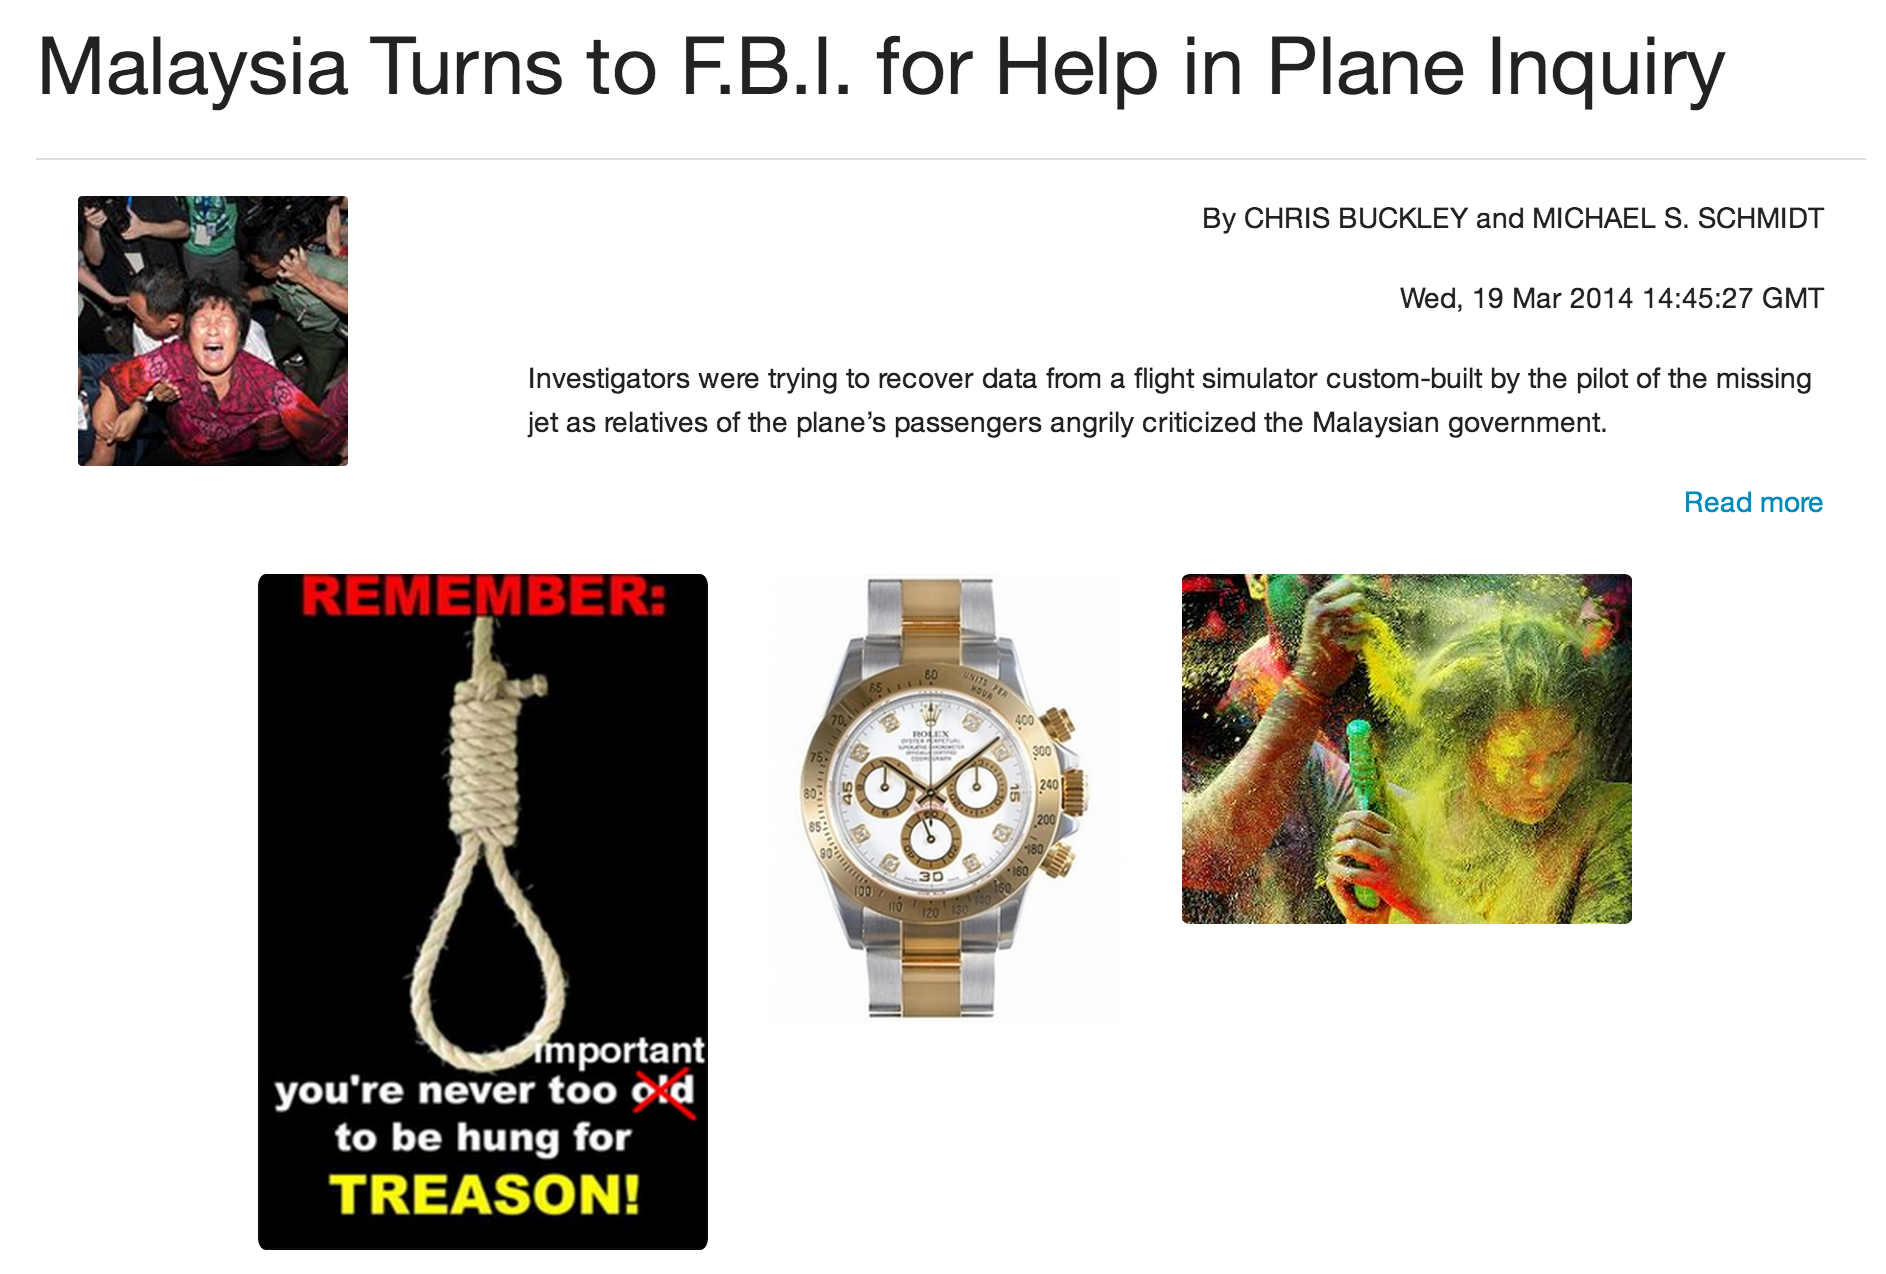
\includegraphics[width=0.9\linewidth]{img/limitation-ZK.png}
  \caption{Screenshot demonstrating scenario with photos from Bing, which are off topic}
  \label{screenshot:limitation}
\end{figure}

\begin{table}[!ht]
  \centering
  \caption{Summary search results for the term 'Malayisia' - most referenced urls in tweets with the given search topic, and urls with most positive/negative connotations}
    \label{table:summaryresults}
    \begin{tabular}{| l | l | l |}
	Source & Title & Count  \\ \hline
	\textbf{Most popular tweets} & \multicolumn{2}{c}{}  \\ \hline 
   masarif.in & Malaysia Airlines, Hilang atau 'Disembunyikan'? & 2667 tweets  \\ 
   dailykeynews.com & Malaysia Flight 370 Hijacked: Investigation Officials Confirm & 400 tweets \\
   dailykeynews.com & Startling Revelations about Malaysia Airlines flight MH370! & 265 tweets \\
  \textbf{Positive connotation} & \multicolumn{2}{c}{} \\ \hline 
   www.trending.co.ke & Malaysia Airlines ad &31\% tweets positive \\
   dailymail.co.uk & Queen of Malaysia from enjoying a round of golf & 10\% tweets positive  \\ 
   hai-online.com & KEMBALI MANGGUNG DI MALAYSIA, EPONK ... & 5.7\% tweets positive \\
   \textbf{Negative connotation} & \multicolumn{2}{c}{} \\ \hline 
   edition.cnn.com & Flight 370 search area shifts after 'credible lead' & 100\% tweets negative \\
   bbc.com & Flight MH370: Bad weather again hampers plane search & 100\% tweets negative \\
   abcnews.go.com & Search for Missing Malaysia Airlines Plane Shifts Northeast & 73\% tweets negative \\
  \end{tabular}
\end{table}

\begin{table}[!ht]
  \centering
  \caption{Tweeted links pertaining to cluster 1 (major topic - search for the plane)}
    \label{table:linkscluster1}
    \begin{tabular}{| l | l |}
	Source & Title \\ \hline
cbsnews.com & Malaysia Airlines Flight 370: China demands satellite data\\
news.com.au & Thai satellite spots 300 objects possibly part of missing plane\\
linkis.com & Data recorder batteries of Malaysia Airlines Flight 370 could already be dead\\
  \end{tabular}
\end{table}

\begin{table}[!ht]
  \centering
  \caption{Tweeted links pertaining to cluster 2 (major topic - Malaysia Ferrari 2014)}
    \label{table:linkscluster}
    \begin{tabular}{| l | l |}
	Source & Title \\ \hline
skysports.com & Sky Sports F1's ... look ahead to the Petronas Malaysia GP \\
sidepodcast.com & Race information - Malaysia 2014\\
formula1.com & Malaysia preview - teams set to feel the heat in Kuala Lumpur\\
  \end{tabular}
\end{table}

\ref{screenshot:cluster1}
\begin{figure}[H]
  \centering
  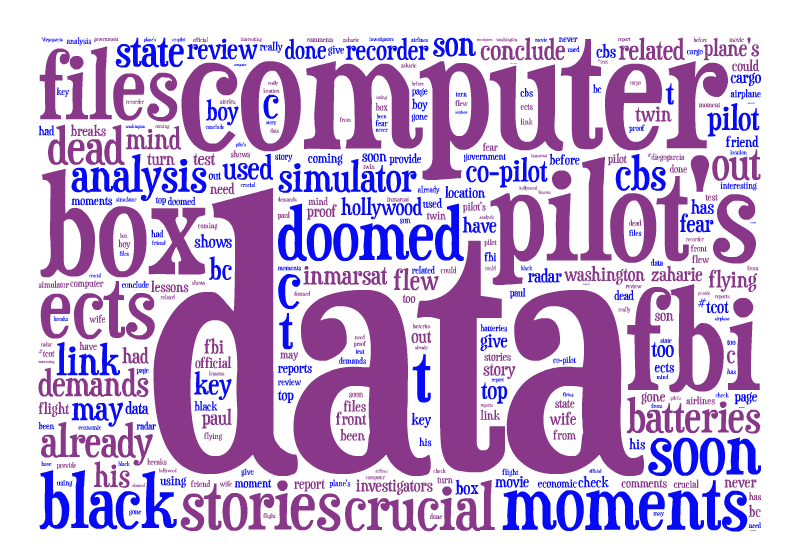
\includegraphics[width=0.9\linewidth]{img/cluster1.png}
  \caption{Word cloud for cluster of tweets concerning Malaysia airplane crash}
  \label{screenshot:limitation}
\end{figure}

\ref{screenshot:cluster2}
\begin{figure}[H]
  \centering
  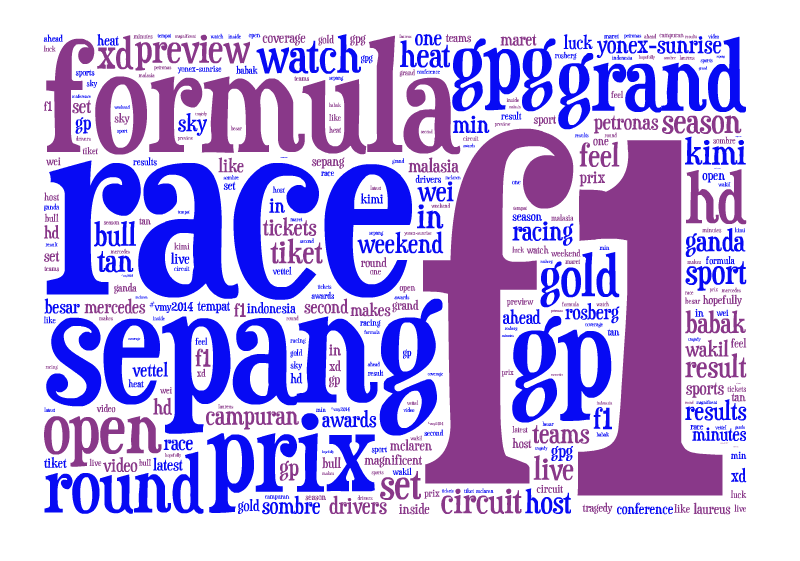
\includegraphics[width=0.9\linewidth]{img/cluster2.png}
  \caption{Word cloud for cluster of tweets concerning upcoming Malaysia formula 1 competition}
  \label{screenshot:limitation}
\end{figure}


% ***********************************************************************
%                           SOME USEFUL EXAMPLES

% Footnote && Caption
% "\textbf{Where in the World Are the Hottest Social Networking Countries?}"
% \footnote{http://www.emarketer.com/Article/Where-World-Hottest-Social-Networking-Countries/1008870}
% \textit{emarketer}

%CITATION
%\citeA{mccombs1972agenda}
% \cite{wanta2004agenda}

% UNFORMATTED CODE EXAMPLE
% \begin{verbatim}
%  {
%     "text": "Russia's 25,000-troop...",
%     "urls": [
%         {
%             "url": "http://rt.com/news/r...",
%             "country_code": "RU"
%         }
%     ],
%     "country_code": "SK"
% }
% \end{verbatim}

% FIGURES
% \ref{screenshot:sentimentmap}
% \begin{figure}[H]
% 	\centering
% 	\includegraphics[width=0.9\linewidth]{crimea_sentiment.png}
% 	\caption{Sentiment analysis}
% 	\label{fig:sentimentmap}
% \end{figure}


\end{document}